\documentclass{beamer}

\usetheme{CambridgeUS}
\usefonttheme{professionalfonts}

\usepackage{graphicx}
\usepackage[miktex]{gnuplottex}
\ShellEscapetrue
\usepackage{epstopdf}
\usepackage{minted}
\usepackage{xcolor}

\usemintedstyle{manni}
\definecolor{mintedBg}{rgb}{0.98,0.98,0.70}

\begin{document}
\title{Automatic differentiation beyond typedef and operator overloading}
\author{Peter Caspers}
\institute{Quaternion Risk Management}
\date{November 30, 2015}

\frame{\titlepage}

\frame{\frametitle{Table of contents}\tableofcontents[hideallsubsections]}

\section{Introduction to AD}

\begin{frame}[fragile]
\frametitle{AD in a nutshell 1/3}
\begin{itemize}
\item for a computer program $f:\mathbb{R}^n\rightarrow\mathbb{R}^m$, compute $\partial_{x} f$
\item $...$ by looking at the program's sequence of basic operations ($+-*/, \exp ...$) and using basic calculus in each step
\item $...$ and stitching everything together with the \textcolor{purple}{chain rule}
\end{itemize}
\end{frame}

\begin{frame}[fragile]
\frametitle{AD in a nutshell 2/3}
\begin{itemize}
\item results are exact up to machine precision, also for higher order derivatives
\item implementation: \begin{itemize}
\item operator overloading instrumenting the double type\footnote{e.g. CppAD, ADOL-C, Adept, dco, proprietary tools}
\item source code transformation tools\footnote{e.g. ADIC, OpenAD/F}
\item coding by hand
\end{itemize}
\end{itemize}
\end{frame}

\begin{frame}[fragile]
\frametitle{AD in a nutshell 3/3}
\begin{itemize}
\item local jacobians can be propagated forward ($x\leadsto y$) (that's intuitive)  or backward \footnote{\tiny\url{https://quantlib.wordpress.com/2015/08/09/backward-automatic-differentiation-explained/}} ($y\leadsto x$) in a dual or \textcolor{purple}{\textit{adjoint}} fashion
\item one \textit{forward} sweep yields one directional derivative of your choice of the vector of output variables
\item one \textit{reverse} sweep yields the gradient w.r.t. all input variables of one linear combination of the output variables
\item the complexity for one (forward or reverse) sweep is a constant, low multiple of the complexity for one function evaluation\footnote{theory tells us that the multiple in adjoint mode is bounded by 4}
\item in particular: \textbf{law of cheap gradient} !
\end{itemize}
\end{frame}

\begin{frame}[fragile]
\frametitle{Adjoint mode example}
\begin{itemize}
\item program $f:\mathbb{R}^n\rightarrow\mathbb{R}$: $y = \exp\left( \prod_{i=0}^n x_i \right) \sin\left( \prod_{i=0}^n x_i \right)$
\item imagine $n$ to be large, like $1000$
\item evaluation complexity: $n+4=\textcolor{purple}{O(n)}$ operations $\in \{*, \exp, \sin \}$
\item goal: compute $\partial_x f \in \mathbb{R}^n$
\item finite difference approach: $(n+1)(n+4) = \textcolor{purple}{O(n^2)}$ operations in addition to the evaluation
\end{itemize}
\end{frame}

\begin{frame}[fragile]
\frametitle{Adjoint mode example - distance 1 nodes}
\begin{itemize}
\item init $\partial_y y = 1$
\item first break down is $y = u*v$, $u=\exp\left( \prod_{i=0}^n x_i \right)$, $v=\sin\left( \prod_{i=0}^n x_i \right)$
\item $\partial_u y = v$, $\partial_v y = u$
\item $2$ operations assuming we have performed a forward sweep, so we
\begin{itemize}
\item know the value of $u$ and $v$ and
\item have built the computational graph and
\item know the ``analytics'' for the local derivatives
\end{itemize}
\item we are not overly pedantic on how to count the operations in this example here ...
\end{itemize}
\end{frame}

\begin{frame}[fragile]
\frametitle{Adjoint mode example - distance 2 nodes}
\begin{itemize}
\item second break down $u = \exp(x), v= \sin(x)$
\item $\partial_x u = \exp(x), \partial_x v = \cos(x)$
\item $\partial_x y = \partial_u y \partial_x u + \partial_v y \partial_x v = \sin(x)\exp(x)+\exp(x)\cos(x)$
\item again, we know $x$ from the forward sweep
\item $5$ operations (total operations count $7$)
\end{itemize}
\end{frame}

\begin{frame}[fragile]
\frametitle{Adjoint mode example - distance 3 nodes}
\begin{itemize}
\item third break down $x = x_0 h_0$
\item $\partial_{x_0} x = h_0, \partial_{h_0} x = x_0$
\item $\partial_{x_0} y = \partial_x y \partial_{x_0} x = [\sin(x)\exp(x)+\exp(x)\cos(x)] h_0$
\item $\partial_{h_0} y = \partial_x y \partial_{x_0} h_0 = [\sin(x)\exp(x)+\exp(x)\cos(x)] x_0$
\item ... we know $h_0$ from the forward sweep ...
\item $4$ operations (total operations count $11$)
\end{itemize}
\end{frame}

\begin{frame}[fragile]
\frametitle{Adjoint mode example - nodes with distance n+2}
\begin{itemize}
\item continue like in the third break down until we arrive at $h_{n-1} = x_n$
\item $\partial_{x_i} y = [\sin(\prod x_i)\exp(\prod x_i)+\exp(\prod x_i)\cos(\prod x_i)] \prod_{j\neq i} x_i$
\item $4(n-2)$ operations from the third break down on
\item total operations count $4(n-2)+7 = \textcolor{purple}{4n-1}$
\item one function evaluation was $\textcolor{purple}{n+4}$ operations
\item naive approach for gradient calculation was $\textcolor{purple}{(n+1)(n+4)}$ operations
\end{itemize}
\end{frame}

\frame{\frametitle{Table of contents}\tableofcontents[hideallsubsections]}

\section{Approaches in QuantLib}

\begin{frame}[fragile]
\frametitle{The typedef approach}
\begin{itemize}
\item just says \verb+typedef CppAD::AD<double> Real+
\item it is a bit more complicated than that
\item QuantLibAdjoint (CompatibL), with additional logic (tapescript)
\item \textit{AD-or-not-AD} decision at compile time and globally, i.e. no selective activation of variables
\end{itemize}
\end{frame}

\begin{frame}[fragile]
\frametitle{Matrix multiplication with (sleeping) active doubles}
\begin{minted}[bgcolor=mintedBg,fontsize=\footnotesize]{c++}
    Matrix_t<T> A(1024, 1024);
    Matrix_t<T> B(1024, 1024);
    ...
    Matrix_t<T> C = A * B;
\end{minted}
\begin{itemize}
\item \verb+T = double+: 764 ms
\item \verb+T = CppAD::AD<double>:+ 8960 ms
\item penalty: 11.7x
\item note that we do not get anything for that (AD is disabled)
\item this is not an exception, but seems to occur for every ``numerically intense'' code section (see below for a second example)
\end{itemize}
\end{frame}

\begin{frame}[fragile]
\frametitle{Active doubles vs. native doubles 1/2}
\begin{itemize}
\item for a \verb+MinimalWrapper+ consisting of a \verb+double+ and a pointer \verb+MinimalWrapper*+ (set to \verb+nullptr+ always), the penalty is around 2.1x
\item for this gcc generates \textit{scalar} double instructions (\textcolor{blue}{mulsd}, \textcolor{blue}{addsd})
\item for the native \verb+double+ gcc generates \textit{packed} double instructions (\textcolor{blue}{mulpd}, \textcolor{blue}{addpd})
\item in addtion the more involved data layout of the \verb+MinimalWrapper+ (placing a pointer after each native \verb+double+) leads to more instructions in the innermost loop
\end{itemize}
\end{frame}

\begin{frame}[fragile]
\frametitle{Active doubles vs. native doubles 2/2}
\begin{itemize}
\item (current) compilers seem to generate more instructions and possibly less efficient instructions for non-native double wrappers
\item memory consumption will go up, too
\item it is not clear what the ``best possible'' OO tool can achieve, but probably it will be something between 2x and 12x
\item 2x is already too much, if we do not get anything for that
\item we can easily avoid this useless overhead
\end{itemize}
\end{frame}

\begin{frame}[fragile]
\frametitle{The template approach}
\begin{itemize}
\item introduce templated versions of relevant classes (e.g. \verb+Matrix_t+)
\item for backward compatibility, \verb+typedef Matrix_t<Real> Matrix+
\item it is a bit more complicated than that
\item allows mixing of active and native classes, as required, i.e. activation of variables in selected parts of the application only
\item work in progress\footnote{conversion rate $\approx$ 2000 LOC / day (manual + an Elisp-little-helper)}, but basic IRD stuff works (like yield and volatility termstructures, swaps, CMS coupons, GSR model)
\item \footnotesize \url{https://github.com/pcaspers/quantlib/tree/adjoint}
\item \footnotesize \url{https://quantlib.wordpress.com/tag/automatic-differentiation/}
\end{itemize}
\end{frame}

\begin{frame}[fragile]
\frametitle{Expensive gradients with operator overloading}
\begin{itemize}
\item the typedef as well as the template approach use operator overloading tools (like CppAD)
\item for numerically intense algorithms, we observe dramatic performance loss (because less optimization can be applied to non-native types)
\item e.g. a convolution engine for bermudan swaptions is \textbf{80x slower}\footnote{see \tiny\url{https://quantlib.wordpress.com/2015/04/14/adjoint-greeks-iv-exotics}}
in adjoint mode compared to one native-double pricing
\item if AD is actually not needed, the template approach is the way out, otherwise we need other techniques
\end{itemize}
\end{frame}

\frame{\frametitle{Table of contents}\tableofcontents[hideallsubsections]}

\section{Source code transformation}

\begin{frame}[fragile]
\frametitle{Source Code Transformation}
\begin{itemize}
\item generate adjoint code at compile time, which may yield better performance
\item however, does not work out of the box like OO tools
\item no mature tool for C++ (ADIC 2.0 = ``OpenAD/Cpp'' under development)
\item needs specific preparation of code before it can be applied
\end{itemize}
\end{frame}

\begin{frame}[fragile]
\frametitle{OpenAD/F}
\begin{itemize}
\item OpenAD is a language independent AD backend working with abstract xml representations (XAIF) of the computational model
\item OpenAD/F adds a Fortran 90 front end
\item Open Source, proven on large scale real-world models
\item \url{http://www.mcs.anl.gov/OpenAD}
\end{itemize}
\end{frame}

\begin{frame}[fragile]
\frametitle{From QuantLib to SCT}
\begin{itemize}
\item isolate the core computational code and reimplement it in Fortran
\item use OpenAD/F to generate adjoint code, build a separate support library from that
\item use a wrapper class on the QuantLib side to communicate with the support libary
\item minimal library example \footnote{\tiny\url{https://github.com/pcaspers/quantlib/tree/master/QuantLibOAD/simplelib}} and LGM swaption engine\footnote{\tiny\url{https://github.com/pcaspers/quantlib/tree/master/QuantLibOAD/lgm}} available
\item build via \verb+make+ (AD support library) or \verb+make plain+ (without OpenAD - transformation, for testing)
\end{itemize}
\end{frame}

\begin{frame}[fragile]
\frametitle{LGM Bermudan swaption convolution engine}
\begin{itemize}
\item core computation can be implemented in around 200 lines
\item native interface only using doubles and arrays of doubles
\item input: relevant times $\{t_i\}$, model $\{(H(t_i), \zeta(t_i), P(0,t_i)\}$,\\
Termsheet, codified as index lists $\{k_i, l_i, ...\}$
\item output: npv, gradient w.r.t. $\{(H(t_i), \zeta(t_i), P(0,t_i)\}$
\end{itemize}
\begin{minted}[bgcolor=mintedBg,fontsize=\footnotesize]{fortran}
subroutine lgm_swaption_engine(n_times, times, modpar, n_expiries, &
     expiries, callput, n_floats, &
     float_startidxes, float_mults, index_acctimes, float_spreads, &
     float_t1s, float_t2s, float_tps, &
     fix_startidxes, n_fixs, fix_cpn, fix_tps, &
     integration_points, stddevs, res)
\end{minted}
\end{frame}

\begin{frame}[fragile]
\frametitle{Building the AD support library}
\resizebox{\textwidth}{!}{
\begin{minipage}{3.5\textwidth}
\begin{figure}
    \centering
        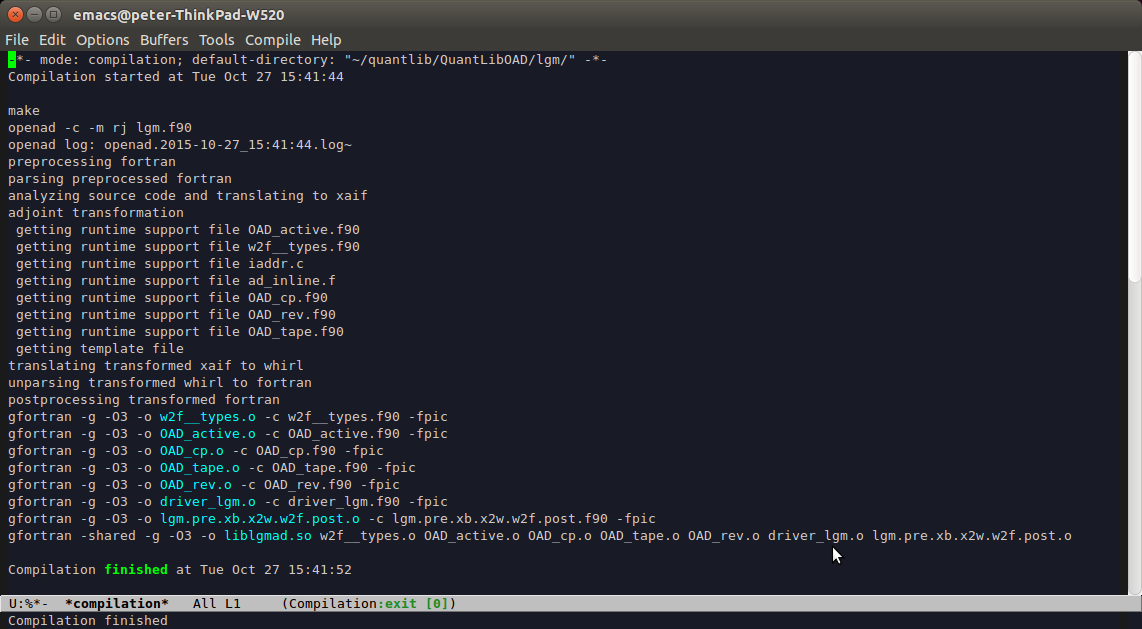
\includegraphics{oad_build.png}
\end{figure}
\end{minipage}}
\end{frame}

\begin{frame}[fragile]
\frametitle{LGM Bermudan swaption convolution engine}
\begin{itemize}
\item C++ wrapper is a normal QuantLib pricing engine
\item precomputes the values and organizes them in arrays for the Fortran core
\item invokes the Fotran routine
\item stores the npv and the adjoint gradient as results
\end{itemize}
\begin{minted}[bgcolor=mintedBg,fontsize=\tiny]{c++}

void LgmSwaptionEngineAD::calculate() const {
    // collect data needed for core computation routine
    ...
    // join all dates and fill index vectors
    ...
    // call core computation routine and set results

    lgm_swaption_engine_ad_(&ntimes, &allTimes[0], &modpar[0], &nexpiries, ...
                    &integration_pts, &std_devs, &res, &dres[0]);
    ...
    results_.value = res;
    results_.additionalResults["sensitivityTimes"] = allTimes;
    results_.additionalResults["sensitivityH"] = H_sensitivity;
    results_.additionalResults["sensitivityZeta"] = zeta_sensitivity;
    results_.additionalResults["sensitivityDiscount"] = discount_sensitivity;
\end{minted}
\end{frame}

\begin{frame}[fragile]
\frametitle{Performance}
\begin{itemize}
\item 10y bermudan swaption, yearly callable
\item 49 grid points per expiry
\item single pricing\footnote{Intel(R) Core(TM) i7-2760QM CPU @ 2.40GHz, using one thread} (non-transformed code): 4.2 ms
\item pricing + gradient $\in \mathbb{R}^{105}$: \textcolor{purple}{\textbf{25.6 ms}}\footnote{to achieve this, the runtime configuration of OpenAD/F has to be modified}
\item additional stuff\footnote{transformation of gradient w.r.t. model parameters to usual vegas, see below}: 6.2 ms
\item adjoint calculation multiple: \textcolor{purple}{\textbf{6.1x}} (7.6x including add. stuff)
\item common, practical target for the adjoint multiple: 5x - 10x
\end{itemize}
\end{frame}

\begin{frame}[fragile]
\frametitle{How not to use AD}
\begin{itemize}
\item avoid to record tapes that go through solvers, optimizers, etc.\footnote{not to be confused with feeding AD - derivatives of the target function to optimizers like Levenberg-Marquardt or Newton-style solvers}
\begin{itemize}
\item instead use the \textcolor{purple}{implicit function theorem} to convert gradients w.r.t. calibrated (model) variables to gradients w.r.t. market variables
\item this is more efficient, less error prone (e.g. \verb+Bisection+ produces zero derivatives always, optimizations may produce bogus derivatives depending on the start value)
\item in the case of SCT applied as above this is even necessary from a practical viewpoint
\end{itemize}
\item apply AD only to differentiable programs (replace a digital payoff for example by a call spread)
\item avoid to record \textit{long} tapes (e.g. for \textit{all} paths of a MC simulation), reuse a tape recorded (in a \textit{tape-safe} way) on one path
\end{itemize}
\end{frame}

\begin{frame}[fragile]
\frametitle{Calibration of LGM model}
To illustrate the usage of the implicit function theorem, consider the calibration to $n$ swaptions\footnote{recall that $\zeta(t)$ is the accumulated model variance up to time $t$}
\begin{eqnarray*}
\text{Black}(\sigma_1) - \text{Npv}_{\text{LGM}}(\zeta_1) &=& 0 \\
... \\
\text{Black}(\sigma_n) - \text{Npv}_{\text{LGM}}(\zeta_n) &=& 0
\end{eqnarray*}
with
\begin{equation}
\frac{\partial \text{Npv}_{\text{LGM}}}{\partial \zeta} = \text{diag}(\nu_1, ..., \nu_n), \text{ all } \nu_i \neq 0
\end{equation}
\end{frame}

\begin{frame}[fragile]
\frametitle{Implicit function theorem}
Locally, there exists a unique $g$
\begin{equation}
g(\sigma_1, ... , \sigma_n) = (\zeta_1, ..., \zeta_n)
\end{equation}
and
\begin{equation}
\frac{\partial g}{\partial \sigma} = \left( \frac{\partial \text{Npv}_{\text{LGM}}}{\partial \zeta} \right) ^ {-1} \frac{\partial \text{Black}}{\partial \sigma}
\end{equation}
\end{frame}

\begin{frame}[fragile]
\frametitle{Pasting the vega together}
\begin{equation*}
\frac{\partial \text{Npv}_\text{Berm}}{\partial \sigma} = \frac{\partial \text{Npv}_\text{Berm}}{\partial \zeta} \frac{\partial \zeta}{\partial \sigma} = \frac{\partial \text{Npv}_\text{Berm}}{\partial \zeta} \left( \frac{\partial \text{Npv}_\text{Calib}}{\partial \zeta} \right) ^ {-1} \frac{\partial \text{Black}}{\partial \sigma}
\end{equation*}
\begin{itemize}
\item the components can be calculated analytically (calibrating swaptions' market vegas) or using the ad engine (calibrating swaptions' $\zeta$-gradient, but this is much cheaper than for the bermudan case)
\item matrix inversion and multiplication is cheap
\item the additional computation time is quite small (see the example above, the addtional costs are the same as for 1.5x original NPV calculations)
\end{itemize}
\end{frame}

\begin{frame}[fragile]
\frametitle{Summary}
\begin{itemize}
\item global instrumentation (via typedefs) with active variables can lead to performance (and memory) issues
\item selective / mixed instrumentation (via templates) solves the issue, but leaves problems when AD is required for numerically intense parts of the code
\item source code transformation can solve this issue, we gave an example in terms of a bermudan swaption engine transformed using OpenAD/F yielding an adjoint multiple of \textbf{\textcolor{purple}{6.1}} compared to \textbf{\textcolor{purple}{80}} with operator overloading (using CppAD)
\end{itemize}
\end{frame}

\frame{\frametitle{Table of contents}\tableofcontents[hideallsubsections]}

\section{Questions}

\begin{frame}[fragile]
\frametitle{Questions / Discussion}
\centerline{Thank you for your attention}
\end{frame}
\end{document}
